\section{\numb section 10. Technical details}

Sections \numb section 10 and \numb section 11 are meant for those intereseted in developing and
extending \maniFEM.
Of course the ultimate documentation is the source code; these sections can be used as
a guide through the source code.


\paragraph{\numb section 10.\numb parag 1. Namespaces and class names}

All names in {\maniFEM} are wrapped into the namespace {\codett maniFEM}.
We recommend {\codett using namespace maniFEM} in your code,
otherwise the text will become cumbersome.
For instance, you will have to write {\codett maniFEM::CellIterator} instead of
{\codett CellIterator}, and so on.
We are {\codett using namespace maniFEM} in the examples of this manual.

As a general rule, namespaces and class names are written with capital initial
letter$\;$:
{\codett Cell}, {\codett Mesh}, {\codett Integrator}, {\codett FiniteElement},
{\codett VariationalFormulation}.
Namespace {\codett tag} (see paragraph \numb section 10.\numb parag 2) is an exception
to the above rule.
Namespace {\codett maniFEM} itself is also an exception, for merely aestetic reasons.

In an effort not to expose too many names in the {\codett maniFEM} namespace, we have
used the namespace {\codett tag::Util} to keep names which did not fit elsewhere.
We have also used anonymous namespaces in order to hide names of functions which are
only used in one file.

In \maniFEM, there are no {\codett private} or {\codett protected} class members or methods.
Everything is {\codett public};
the user can make use of any class member if he or she so chooses.
This can be considered poor design; we endorse this criticism with no further comments.

However, some class members and methods are intended to be used by the final user,
while others are used in the internal implementation of the former.
Classes \hbox{intended} for basic usage are directly exposed in {\codett namespace maniFEM} :
\ {\codett Cell}, {\codett Mesh}, {\codett CellIterator}, \hbox{\codett Function},
{\codett Manifold}, {\codett VariationalFormulation}, {\codett Integrator},
{\codett FiniteElement}, the rarely needed {\codett Field} and the even more rarely needed
{\codett MeshIterator}.
Classes not intended for the final user (at least not for the basic usage of \maniFEM)
have been hidden inside the above mentioned names, e.g. {\codett Mesh::Positive},
\ {\codett CellIterator::Over::SegsOfPosLoop::Positive},
\hbox{\codett Function::CoupledWithField::Scalar}.
Also, in the source code there are comments like

\verbatim
   // do not use directly, let [some other method] do the job
\endverbatim


\paragraph{\numb section 10.\numb parag 2. Tags}

We use extensively {\codett tag}s.
These are structures gathered in the {\codett namespace tag}.
Most of them contain no data; only their type is useful, at compile time.

A {\codett tag} is used to clearly distinguish between functions with the same name
(overloaded functions).
For instance, in the code excerpt below five {\codett CellIterator}s are defined
(by means of the same method {\codett Mesh::iterator}) which
behave very differently (see paragraphs \numb section 8.\numb parag 5 and
\numb section 8.\numb parag 6).

\verbatim
   // 'chain' is a one-dimensional Mesh
   CellIterator it1 = chain.iterator ( tag::over_vertices );
   CellIterator it2 = chain.iterator ( tag::over_vertices, tag::reverse );
   CellIterator it3 = chain.iterator ( tag::over_segments );
   CellIterator it4 = chain.iterator ( tag::over_segments, tag::reverse );
   CellIterator it5 = chain.iterator ( tag::over_segments, tag::force_positive );
\endverbatim

The above could be achieved by giving longer names to the functions, but we believe
{\codett tag}s make the code more readable.
Besides that, in the case of constructors, we do not have the choice of the name of the function
(a constructor has the same name as its class).
{\ManiFEM} uses {\codett tag}s extensively for constructors, e.g.
\verbatim
   Cell A ( tag::vertex );  Cell B ( tag::vertex );
   Mesh AB ( tag::segment, A.reverse(), B, tag::divided_in, 10 );
\endverbatim

In \maniFEM, namespaces and class names begin with capital letter
(see paragraph \numb section 10.\numb parag 1)
The namespace {\codett tag} (or {\codett maniFEM::tag} if you are not
{\codett using namespace maniFEM}) is an exception to the above rule.
We prefer its name to have only lower case letters because we want it to be
discrete. For instance, if we wrote {\codett Tag::divided\_in},
the reader's eye would catch {\codett Tag} much before {\codett divided\_in};
thus, {\codett tag::divided\_in} is more readable.
Of course, the final user has the choice of {\codett using namespace tag}
but beware, it has many names which may conflict with the ones in your code.

Most tags have only lower-case letters and underscores.
The exceptions are proper names : {\codett tag::Lagrange}, {\codett tag::Euclid}.


\paragraph{\numb section 10.\numb parag 3. Wrappers and cores}

Designing and implementing {\maniFEM} has been a challenging endeavour.
We had a lot of fun and we have learned much along the process.

Take cells and meshes, for instance.
As explained in paragraph \numb section 1.\numb parag 2, at the conceptual level meshes
are roughly collections of cells of the same dimension and cells are essentially
defined by their boundary which is a lower-dimensional mesh.
This conceptual simplicity does not survive to the demands of an efficient code
(although it has been extremely useful in the process of designing \maniFEM;
it should also be useful for learning and using it).

Vertices (zero-dimensional cells) have no boundary at all.
One-dimensional cells (segments) have all the same shape and have a rudimentary boundary
(a zero-dimensional mesh consisting of a {\codett base} and a {\codett tip}).
In order to save space in the computer's memory, specific classes have been created for
vertices and for segments.

Also, there are positive cells and negative cells, positive meshes and negative meshes.
A positive cell and its negative counterpart (its {\codett reverse}) share some information.
To save memory space, negative cells are implemented in different classes from
positive cells, thus avoiding the storage of some of the redundant information.

We want, however, to manipulate all these different cells through a uniform interface,
which is where {\tt C++}'s inheritance and polymorphishm mechanisms come handy.
Thus, there are classes {\codett Cell::Positive::Vertex}, {\codett Cell::Positive::Segment}
and {\codett Cell::Positive}, all derived from {\codett Cell::Core::Positive}.
And we have {\codett Cell::Negative::Vertex}, {\codett Cell:: ::Negative::Segment} and {\codett
Cell::Negative}, all derived from {\codett Cell::Core::Negative}.
Both {\codett Cell::Core::Positive} and {\codett Cell::Core::Negative} are derived from
{\codett Cell::Core}.

On the other hand, we want cells and meshes to be persistent objects (not subject to
syntactic scope).
We create them within some function and we want them to remain alive after returning
to the main program.
Also, they are unique entities, it does not make sense to copy them.
This is why we have implemented {\codett Cell} as a thin wrapper around {\codett Cell::Core}
with most methods of {\codett Cell} being delegated to {\codett Cell::Core}.
When it goes out of its syntactic scope, the wrapper is destroyed but the {\codett Cell::Core}
object inside remains intact.
Also, you can copy the wrapper as in {\codett Cell A = B} or {\codett Mesh BA = AB.reverse()}
but these operations do not create new core objects, they just give new names to
already existing cells or meshes (Paragraph \numb section 8.\numb parag 10 gives more details).
You can think of {\codett Cell}s and {\codett Mesh}es as customized pointers towards
{\codett Cell::Core}s and {\codett Mesh::Core}s, respectively.

Negative meshes contain no useful information (they only appear as boundaries
of negative cells) so there is no such class as {\codett Mesh::Negative}.
All {\codett Mesh::Core}s are positive.
The wrapper class {\codett Mesh} contains a pointer to a {\codett Mesh::Core} and a flag
telling it to reverse everything if the mesh is to be considered negative.
Zero-dimensional meshes (boundaries of segments) are not stored at all.
One-dimensional meshes have a specific structure (they are chains of segments)
and will receive in the future a specific treatment (a specialized class).

To save memory, we don't even keep the dimension of a cell as an attribute,
it's a static property for vertices and segments, while for higher-dimensional cells
it's obtained from the boundary's dimension.
The dimension of a mesh is not kept as an attribute either; it's computed on-the-fly
by counting the levels of collections of cells the mesh is made of (and then
substracting one).
For instance, the mesh in paragraph \numb section 1.\numb parag 1 has three layers of cells :
points, segments and squares.

Constructors for wrapper classes act as factory functions for the core object.
According to their arguments, they build different core objects.

Other objects have been implemented using the same logic of wrappers and core objects.
Iterators, fields, functions, manifolds.

% There are Euclidian manifolds, cartesian products, implicitly defined submanifolds and
% parametrized submanifolds.
% Distinct notions with very different internal implementations.
% But we would like to offer the user the possibility of declaring any of these as ``a
% {\codett Manifold}''.


\paragraph{\numb section 10.\numb parag 4. The lifecycle of objects}

Many objects in {\maniFEM} are implemented using a wrapper-core model.
Examples are {\codett Cell}s, {\codett Mesh}es, {\codett CellIterator}s, {\codett MeshIterator}s,
{\codett Manifold}s, {\codett Function}s, {\codett FiniteElement}s, {\codett Integrator}s,
{\codett VariationalFormulation}s.
A garbage collector is implemented; all these classes inherit from {\codett tag::Util::Wrapper}
and their cores inherit from {\codett tag::Util::Core}.
Wrappers contain a pointer to a core; each core keeps a counter of wrappers pointing to it.
The destructor of a wrapper decrements the counter and destroys the core if the counter
reaches zero.
It's like a {\codett shared\_ptr}.

Cells and meshes depend on each other in a complicated manner.
A cell keeps its boundary (which is a mesh) alive.
A mesh keeps its component cells alive.
A negative cell keeps alive its positive counterpart but the reverse does not hold;
care must be taken to break dependency cycles.

Some programs consist only in building a mesh and never destroying cells.
For such programs, there is no advantage in using a {\codett shared\_ptr}-like strategy.
Thus, unlike for other {\maniFEM} objects, the garbage collector for {\codett Cell}s and
{\codett Mesh}es can be turned off by erasing the option {\codett -DMANIFEM\_COLLECT\_CM}
in the {\codett Makefile}.
Remember to {\codett make clean} and re-build your program.
If you turn off the garbage collector, {\codett Cell}s and {\codett MMesh}es will occupy
less space in the computer's memory and your program will run slightly faster.
You should not do this if you do remeshing, or ghost cells and meshes will fill
the computer's memory.


\paragraph{\numb section 10.\numb parag 5. \special{ps: gsave 0.6 setgray}Different kinds of meshes\special{ps: grestore}}

{\bf This paragraph describes an implementation of meshes
not yet included in the {\codett master} branch of \maniFEM.
It should be regarded as an early announcement of the new implementation.}

A {\codett Mesh} wrapper contains a pointer to a {\codett Mesh::Core}.
The latter is a polymorphic object; there are several different kinds of meshes
which differ in their internal implementation; the wrapper provides a uniform interface
to the user (making use of the virtual methods of the core).

Negative meshes are temporary wrappers built on-the-fly.
Their core points to a positive mesh.

Zero-dimensional meshes appear only as boundaries of segment {\codett Cell}s.
They are temporary objects built on-the-fly.

Some meshes are implemented as {\codett Mesh::Fuzzy}.
They have as attributes lists of cells of different dimensions;
these lists have no particular order.
Iterators over cells of {\codett Fuzzy} meshes simply run over the respective lists of cells.

Other meshes are assumed to be connected and keep no lists of cells.
Iterators over such meshes traverse the mesh beginning at a starting point (which is an
attribute of class {\codett Mesh::Connected::***Dim}) and then using the neighbourhood relations
to move from one cell to another.

One-dimensional connected meshes are a special case because their topology is peculiar;
segments and vertices composing such a mesh have a natural order (linear order).
Recall that all meshes in {\maniFEM} are oriented.
A one-dimensional connected mesh can be a closed loop or an open chain of segments.
In the latter case, there is a natural starting point (the first vertex or first segment).
Iterators over such meshes are described in paragraph \numb section 8.\numb parag 6.
The {\codett Mesh} constructor with {\codett tag::segment} builds an open
{\codett Mesh::Connected::\break ::OneDim}.
Also, cell constructors with {\codett tag::triangle} and {\codett tag::quadrangle} produce cells
whose boundary is a closed {\codett Mesh::Connected::OneDim}.

Connected meshes of dimension two or higher are not yet implemented; for now,
constructors with {\codett tag::rectange} or {\codett tag::triangle} build a
{\codett Fuzzy} mesh instead.
A class {\codett Mesh::Connected::HighDim} is object of current work.
We also intend to implement multiply connected meshes.
% Implementing classes\break {\codett Mesh::MultiplyConnected::OneDim} and
% {\codett Mesh::MultiplyConnected::HighDim} is a long-term goal.

Iterators over cells of a {\codett Fuzzy} mesh are fast because they simply run over the
list of cells of given dimension.
Iterators over {\codett Connected} meshes may be slower because they traverse the mesh using
neighbourhood relations between cells.
On the other hand, {\codett Fuzzy} meshes require more space in the computer's memory.

The kind of a certain mesh is not always completely obvious.
For instance, when {\codett join}ing two meshes of the kind {\codett Mesh::Connected::OneDim},
the result will be a\break {\codett Mesh::Connected::OneDim} if the last vertex of one of the meshes
is the same as the first vertex of the other one.
Otherwise, the result will be a {\codett Mesh::Fuzzy}.
\vfil\eject


\paragraph{\numb section 10.\numb parag 6. Maximum topological dimension}

\leavevmode {\ManiFEM} assumes you will not build meshes of topological dimension
above 3.
If you want to play with higher-dimensional meshes, you must relax this assumption
through the statement {\codett Mesh::set\_max\_dim (}some-integer{\codett )}.

On the other hand, you may want to decrease the expected dimension.
Suppose you want to mesh surfaces in $ \RR^3 $.
This means your maximum topological dimension will be 2
(this has nothing to do with the geometric dimension, here 3).
Then you may state your intention at the beginning of your program
(before building any cell, before even declaring the first vertex) through
the statement {\codett Mesh::set\_max\_dim(2)}.
This will decrease the size of the {\codett Cell::Core} objects in your code,
thus saving some memory.

But beware, if you try to build a mesh of dimension higher than the one expected by
\maniFEM, you will get an {\codett assertion error} at run-time in {\codett DEBUG} mode,
or some bizarre behaviour (often a {\codett segmentation fault}) in {\codett NDEBUG} mode.
The {\codett DEBUG} mode is explained at the beginning of paragraph \numb section
10.\numb parag 13.


\paragraph{\numb section 10.\numb parag 7. Declaring cell cores}

As explained in paragraph \numb section 10.\numb parag 3, the {\codett Cell} class is
just a thin wrapper around a {\codett Cell::Core}.
While it is possible and useful to copy {\codett Cell}s (think of them as customized
pointers to {\codett Cell::Core}s), objects in the {\codett Cell::Core} class cannot be copied.
Statements below will produce a compilation errror.

\verbatim
   Cell::Core A ( B );  //  B is a Cell::Core
   C = D;  //  C and D are Cell::Core objects
\endverbatim

Objects in the {\codett Cell::Core} class have an attribute {\codett reverse\_p}
which is {\codett nullptr} if the cell has no reverse (yet), otherwise points to the
reverse core cell.
Note that negative cells must have a reverse, which is a positive cell.
Positive cells may have no reverse.

{\codett Cell::Core}s have a method method {\codett reverse}, which requires a
{\codett tag::build\_if\_not\_exists} as argument.
It behaves similarly to the method {\codett reverse} in class {\codett Cell},
described in paragraph \numb section 8.\numb parag 10.
That is, a reverse {\codett Cell::Core} object is built on-the-fly if needed :

\verbatim
   Cell::Core * rev_cll_p = cll_p->reverse ( tag::build_if_not_exists );
   assert ( rev_cll_p );
\endverbatim

Recall that reverse meshes exist always (negative meshes are temporary objects built
on-the-fly).

Methods {\codett cell\_behind} and {\codett cell\_in\_front\_of} in class {\codett Mesh}
also accept a pointer to a {\codett Cell::Core} as an argument.
When the {\codett tag::may\_not\_exist} is provided,
they return a pointer towards the respective neighbour cell, if it exists, otherwise
they return {\codett nullptr}.

\verbatim
   Mesh msh ( ... );  // some constructor
   Cell::Core * f_p = ... ;  //  f_p points to a face within msh
   Cell::Core * cll_p = msh.cell_in_front_of ( f_p, tag::may_not_exist );
   if ( cll_p ) do_something_to ( *cll_p );
   else cout << "no neighbour !" << endl;
\endverbatim

When the {\codett tag::surely\_exists} (or no tag at all) is provided as an argument,
they return a pointer to an existing cell :

\verbatim
   Cell::Core * cll_p = msh.cell_in_front_of ( f_p, tag::surely_exists );
   // or, equivalently :
   Cell::Core * cll_p = msh.cell_in_front_of ( f_p );

   // first_vertex, last_vertex, first_segment, last_segment
\endverbatim

This version of {\codett cell\_behind} and {\codett cell\_in\_front\_of} should be
slightly faster than the one with {\codett tag::may\_not\_exist}.
However, you should only use it when you are confident that the neighbour cell already
exists.
Otherwise, an {\codett assertion error} will occur in {\codett DEBUG} mode;
in {\codett NDEBUG} mode, the behaviour is undefined (often, a {\codett segmentation fault}
will arise).
The {\codett DEBUG} mode is explained at the beginning of paragraph \numb section
10.\numb parag 13.

Paragraph \numb section 8.\numb parag 10 explains similar operations on wrapper classes
{\codett Cell} and {\codett Mesh}.


\paragraph{\numb section 10.\numb parag 8. Disposing of meshes}


In paragraph \numb section 1.\numb parag 3 and others we have shown how to {\codett join} meshes.
The question arises, do we need to keep the intermediate meshes or just the final, big, one ?
That's up to the user to decide. If we prefer to keep only the final mesh, we can ``get rid''
of the meshes we don't need anymore by means of the method {\codett dispose}.

Note that it is not enough for the respective {\tt C++} object to go out of scope.
In \maniFEM, cells and meshes are created on the free store and survive outside their
syntactic scope (see paragraph \numb section 10.\numb parag 3).
The user must release them explicitly.

For instance, in paragraph \numb section 1.\numb parag 3, after building {\codett L\_shaped},
we may add the following lines of code :

\verbatim
   BC.dispose();  // BC.reverse() will be discarded, too
   CD.dispose();  // CD.reverse() will be discarded, too
   ABCD.dispose();  CEFD.dispose();  BGHC.dispose();
\endverbatim

The {\codett dispose} operation will only discard component cells which belong to no other
mesh.
The {\codett shread} method can be used to forcefully discard all cells in the mesh,
but the need for such should be rare.


\paragraph{\numb section 10.\numb parag 9.
\special{ps: gsave 0.6 setgray}About {\tt init\_cell}\special{ps: grestore} (outdated)}


The {\codett Cell} class has static attributes {\codett init\_cell}, {\codett init\_cell\_r},
{\codett data\_for\_init}, {\codett data\_for\_init\_r}.
The attribute {\codett init\_cell} is a list of pointers to functions to be called by
the constructor of a positive cell, while {\codett data\_for\_init} is a void pointer which
can be used to pass supplementary information to {\codett init\_cell}.
Attributes {\codett init\_cell\_r} and {\codett data\_for\_init\_r} fulfill a similar task
when building negative cells.

For instance, {\codett Manifold::coordinate\_system} inserts into the list
{\codett Cell::init\_cell[0]} a call to {\codett Mesh::prescribe\_on} which in turn calls
{\codett FunctionOnMesh::prescribe\_on} in order to prepare the ground for instructions like
{\codett x == 1.0} to produce the desired effect after the creation of each point.

Another example is the constructor {\codett FiniteElement::Lagrange::Q1}
which adds a call to {\codett FiniteElement::Lagrange::Q1::enumerate\_new\_vertex} to
the list {\codett Cell::init\_cell[0]}.
This way, future vertices will receive automatically a {\codett size\_t} label, to be used
by Lagrange finite elements.


\paragraph{\numb section 10.\numb parag 11. Programming style}

I (Cristian) have chosen some program-writing conventions which may seem unusual for other people.
For instance, most programmers use braces like this

\verbatim
   for ( ... ) {
      statement 1;
      statement 2;
      statement 3;
   }
\endverbatim

or perhaps like this

\verbatim
   for ( ... )
   {
      statement 1;
      statement 2;
      statement 3;
   }
\endverbatim

I just can't accept the idea that a brace opens more to the right that it closes, or at the
same point.
For me, a pair of braces should open at some point to the left and close at some point to the
right, and the statements should be between them.
That's how parentheses have been designed to be used.
So I irreverently decided that my blocks will look like this.

\verbatim
   for ( ... )
   {  statement 1;
      statement 2;
      statement 3;  }
\endverbatim

I am aware I am violating conventions which are almost universally accepted. Sorry about that.

On the other hand, I am very fussy about indentation.
I guess my mind has been formatted by Python.

{\codett CellIterator}s obey to syntactic rules slightly different from the conventions for
iterators in the Standard Template Library.
See paragraph \numb section 8.\numb parag 5.

Also, the version numbering is somewhat unusual.
The version consists merely of the year and month.
Perhaps a nostalgic memory of my first serious programming language, FORTRAN 77 ?


\paragraph{\numb section 10.\numb parag 12. Frequent errors at compile time}

\verbatim
variable [name] set but not used [-Wunused-but-set-variables]
[name] defined but not used [-Wunused-function]
\endverbatim

These are harmless warnings.

Some variables are initialized but never used.
When we create a {\codett Manifold}, the constructor sets a global variable
{\codett Manifold::current}.
Thus, {\maniFEM} can remember at any time the geometry of the space and it can choose the right
interpolation and projection operations.
From the compiler's viewpoint, that {\codett Manifold} oject is never used again and so it issues
a warning.

Also, some functions are never used.
They are there mainly for historical reasons.
They have not been erased yet because part of their code may still be used in the future.


\verbatim
'class ManiFEM::Cell::Core' has no member named 'name'
-- or --
'class ManiFEM::Cell::Core' has no member named 'get_name'
\endverbatim

It seems you are trying to compile your code in {\codett NDEBUG} mode (see the beginning
of paragraph \numb section 10.\numb parag 13).
In {\codett NDEBUG} mode, cells and meshes do not have names.

\verbatim
cannot declare variable 'cll' to be of abstract type 'ManiFEM::Cell::Core'
-- or similar for PositiveBaseCell or NegativeBaseCell or CoreMesh --
\endverbatim

Classes {\codett Cell::Core}, {\codett PositiveBaseCell} and
{\codett NegativeBaseCell} are abstract and cannot be instantiated.
You must be more specific; {\codett PositiveVertex}, {\codett NegativeVertex},
{\codett PositiveSegment}, {\codett NegativeSegment}, {\codett PositiveCell} and
{\codett NegativeCell} can be instantiated.

\verbatim
use of deleted function 'ManiFEM::PositiveVertex& ManiFEM::
PositiveVertex::PositiveVertex(const ManiFEM::PositiveVertex&)'
-- or similar for NegativeVertex or PositiveSegment or NegativeSegment --
--      or PositiveCell or NegativeCell or PositiveMesh --
-- or --
use of deleted function 'ManiFEM::PositiveVertex& ManiFEM::
PositiveVertex::operator=(const ManiFEM::PositiveVertex&)'
-- or similar for NegativeVertex or PositiveSegment or NegativeSegment --
--      or PositiveCell or NegativeCell or PositiveMesh or PosOneDimMesh --
\endverbatim

Core cells and meshes cannot be copied.
You cannot ask for things like {\codett cell\_2 = cell\_1} or {\codett mesh\_2 =
mesh\_1}.
See paragraph \numb section 10.\numb parag 7 for more details.


\paragraph{\numb section 10.\numb parag 13. Frequent errors at run time}

Some errors give explicit messages. For instance :

\verbatim
only one-dimensional meshes have first vertex
-- or --
ManiFEM::Cell& ManiFEM::Cell::tip(): Assertion 'dim == 1' failed.
\endverbatim
\smallskip

When you think your program is ready for shipping, you may want to speed it up
by adding the {\codett -dNDEBUG} option to your compilation command
(check your {\codett Makefile}).
You may want to add other optimization options like {\codett -O2}.
Remember to {\codett make clean} before re-building your application.

If your program produces unpredictible, random errors at run-time, e.g.\ throws
{\codett segmentation fault}, try running it in debug mode.
To achieve this, simply remove any {\codett -dNDEBUG} option from your compilation
command (check your {\codett Makefile}).
Remember to {\codett make clean} before re-building your application.

Errors described below are produced by {\codett assert}ions and thus will
only show up in {\codett DEBUG} mode.

\smallskip\verbatim
ManiFEM::Cell& ManiFEM::Cell::base(): Assertion 'dim == 1' failed.
-- or --
ManiFEM::Cell& ManiFEM::Cell::tip(): Assertion 'dim == 1' failed.
\endverbatim

It seems you are trying to get the base or the tip of a cell of dimension
different from $1$.
This does not make sense.

\medskip\verbatim
double& ManiFEM::OneDimField::operator()(ManiFEM::Cell&) const:
Assertion 'cll.real_heap_size() > index_min' failed.
\endverbatim

You probably tried to access a coordinate (or some other value) at a cell to which 
no value has been associated.
Either you picked a cell of a different dimension (e.g.\ a segment instead of a
vertex) or you are looking at a negative cell.
Values are usually stored at positive cells; negative cells have no information attached.
For any cell, you may use the {\codett positive} attribute which is a pointer
equal to {\codett this} if the cell is positive or points to the reverse if
the cell is negative (so the reverse is positive).
Or you may check if a certain cell is positive or negative by using the method
{\codett is\_positive} (which simply returns the result of the comparison {\codett
this == this->positive}).
Paragraph \numb section 8.\numb parag 7 gives more details about orientation of
cells and meshes.
See also paragraphs \numb section 8.\numb parag 10 and \numb section 10.\numb parag 7.

Note that, if {\codett seg} is a segment (a one-dimensional cell), then {\codett
seg.tip()} is a positive cell but {\codett seg.base()} is a negative cell.
So, you probably need to use {\codett seg.base().reverse()} instead.
Iterators over cells of maximum dimension (that is, of dimension equal to the dimension
of the mesh) produce oriented cells (which may be positive or negative).
Consider using the {\codett tag::force\_positive}.
See paragraphs \numb section 8.\numb parag 5 and \numb section 8.\numb parag 6.

\medskip\verbatim
ManiFEM::Cell& ManiFEM::Mesh::cell_in_front_of(ManiFEM::Cell&,
const ManiFEM::tag::SurelyExists&): Assertion 'cll != NULL' failed.
-- or --
ManiFEM::Cell& ManiFEM::Mesh::cell_behind(ManiFEM::Cell&,
const ManiFEM::tag::SurelyExists&): Assertion 'cll != NULL' failed.
\endverbatim

You are navigating dangerously close to the boundary of a mesh.
See paragraph \numb section 8.\numb parag 9.

\medskip\verbatim
static size_t ManiFEM::Mesh::diff(size_t, size_t): Assertion 'a >= b' failed.
-- or --
virtual void ManiFEM::PositiveCell::add_to(ManiFEM::CoreMesh*):
Assertion 'this->meshes.size() > 0' failed.
\endverbatim

You are trying to build meshes of dimension higher than those \maniFEM\ expects.
Did you re-define this expectation through the statement
{\codett Mesh::set\_max\_dim} ?
Along your program, you may have different maximum topological dimensions (that is,
you may use {\codett Mesh::set\_max\_dim} several times) but, at each moment,
you can only build meshes of dimension up to the value most recently defined.
See paragraph \numb section 10.\numb parag 6.
\medskip

If {\tt gmsh} shows an empty drawing, go to {\codett Tools} $\to$ {\codett Options} $\to$
{\codett Mesh}.
For viewing one-dimensional meshes, you need to select {\codett 1D Elements}.


\paragraph{\numb section 10.\numb parag 15. Chains of segments}

One-dimensional meshes are special.
They are mere chains of segments, connected or disconnected.
If they are connected, they may be open chains or closed ones (loops).

We want iterators over cells of one-dimensional meshes to behave orderly.
If the chain is closed, we want the iterator to follow the natural order of the segments.
If the chain is open, we want more, we want the iterator to begin at one end and to go
through until it meets the other end.
These requirements are not compatible with the idea of a disconnected mesh.

So, we have chosen the following solution.
One-dimensional meshes are implemented in class {\codett Mesh::OneDim::Positive} and have
two attributes (which other meshes have not) {\codett first\_ver} and {\codett last\_ver}.
Every time we change a one-dimensional mesh through {\codett add\_to},
{\codett remove\_from}, {\codett glue\_on\_bdry\_of} or {\codett cut\_from\_bdry\_of},
the attribute {\codett first\_ver} of the mesh will be set to {\codett nullptr}.
This means the mesh is in an unordered state.
It may even be disconnected.
This is also the state of a new, empty, mesh.

In the {\codett reset} method of a {\codett CellIterator} over a one-dimensional mesh,
we first check the attribute {\codett first\_ver} of the mesh.
If it is {\codett nullptr}, this means the mesh is unordered, it may even be disconnected.
We then go through all segments and check the structure of the mesh, 
{\codett assert}ing that it is connected, determining whether it is open or closed
and setting accordingly the members {\codett first\_ver} and {\codett last\_ver}.
[implement this in methods {\codett get\_first} and {\codett get\_last}]

If {\codett first\_ver} is equal to {\codett Cell::ghost}, this means that the chain
is closed (it is a loop).
Any other value of {\codett first\_ver} means that the chain is open and that its
ends are stored as {\codett first\_ver} and {\codett last\_ver} and can be used for
initializing the iterator.

The {\codett Cell::ghost} should, of course, not be used for any other purpose.
It is the only negative cell whose {\codett reverse\_p} is {\codett nullptr}.
Its {\codett heap}s have size zero.

A different kind of iterators is under construction.
It will use a {\codett tag::unordered} in its declaration and will behave like an interator
over cells of higher-dimensional meshes, that is, it will not take into account the chain
structure of a one-dimensional mesh.
These {\codett unordered} iterators will accept to run over a disconnected mesh.
Disconnected one-dimensional meshes are used, for instance, in progressive meshing.

In the future, one-dimensional meshes will keep only a list of segments,
without storing the vertices.
Or perhaps not even that, perhaps they will only keep {\codett first\_ver} and
{\codett last\_ver}.


\paragraph{\numb section 10.\numb parag 16. The cloud}

During the mesh generation process described in paragraph \numb section 11.\numb parag 5,
we have to check frequently the distance between
some vertex on the evolving interface and all other vertices of the interface
(including other connected components).
A direct comparison with all vertices would be very time consuming, so we rely on a tree-like
structure which we call {\codett MetricTree} and which eliminates many vertices from the list
of candidates.%
\footnote *{\parbox{\ftntfont\baselineskip=3pt
{\ftnttt MetricTree} is also available separately at
{\ftnttt https://github.com/cristian-barbarosie/MetricTree}}}

The {\codett MetricTree} is similar to quad- and oct-trees with two differences :
there is no assumption on the geometric dimension and the zones overlap.
It is similar to m-trees, just not balanced.

It works for a general metric space.
Triangular inequality is assumed, as well as symmetry.
Because it is not balanced, it deals well with non uniform clouds of points, that is,
with clouds having zones with
high density of points along with zones where the points are spread at large distances.

There is no upper limit on the number of children.
Actually, the average number of children can be used as a hint about the dimension of the
metric space (in the spirit of Hausdorff dimension).

{\codett MetricTree} has been implemented with the intent of having wide usability,
independently of \maniFEM.
It is templated over the type of {\codett Point}s (the metric space) and over a callable
object returning the square of the distance between any two {\codett Point}s.
However, it still needs the touch of someone experienced in the subtleties of {\tt C++}.
Help is welcome.

We focus on the square of the distance rather than on the distance itself because it
is numerically cheaper (we prefer not to compute square roots).
Of course there are parts of the code where the true distance must be used
(e.g. when it comes to the triangular inequality).
Even there, simple algebraic manipulations allow us to avoid computing any square root.

The user interacts with the {\codett MetricTree} through four methods.
The constructor sets the rank-zero distance and the ratio between successive
distances (see below).
Method {\codett add} adds a {\codett Point} to the cloud and returns a pointer to a
{\codett Node} which the user must keep and later provide to the {\codett remove} method.
The {\codett remove} method removes a {\codett Node} from the {\codett MetricTree}.
Finally, and most importantly, method {\codett find\_close\_neighbours\_of} receives a
{\codett Point P} and a distance threshold and returns a list of {\codett Node}s near
{\codett P}.
It is irrelevant whether {\codett P} belongs or not to the cloud (if it belongs, it will
show up in the returned list, disguised as a {\codett Node}).
The user can recover (a copy of) the {\codett Point} from a {\codett Node} using the attribute
{\codett point}.
We have not implemented a method for finding the $n$ nodes closest to a given point
(we do not need such an operation for progressive mesh generation).

It is assumed that {\codett Point}s are cheap to copy.
If this is not the case for your {\codett Point}s, use pointers.
{\ManiFEM} uses wrappers, which are a sort of pointers (see paragraph
\numb section 10.\numb parag 3).

Each node represents a point.
Leaves have no special status.
Each node has a rank which is an integer, possibly zero, possibly negative.
Children of a node {\codett N} have rank equal to {\codett rank[N] - 1}.
Nodes with rank zero have no special status.
Leaves may have any rank, positive, zero or negative.
There is a {\codett root} of course (a node with no parent).
The root has the highest rank.
Even the rank of the root may be negative.

To each rank there is a distance {\codett dist} associated.
Children of a node {\codett N} are no farther than {\codett dist[rank[N]]} from {\codett N}.
Note that a point {\codett P} being at distance less than {\codett dist[rank[N]]} from
{\codett N} does not imply that {\codett P} must be a child (not even an indirect descendant)
of {\codett N}.
In other words : zones overlap.

{\codett dist[k]} is a geometric sequence with ratio {\codett ratio}.
{\codett ratio} must be greater than two; we recommend some value between 5 and 10.
So, {\codett dist[k] == ratio}$^{\hbox{\ftnttt k }}${\codett dist[0]}.
Recall that {\codett k} may be negative.

Besides the {\codett dist}ance, to each rank {\codett k} we associate a {\codett range}
which represents the sum of distances of that rank and of all lower ranks.
That is,
\smallskip\centerline
{{\codett range[k] == dist[k] / ( 1 - 1 / ratio )$\,$}; \ {\codett range[k] > dist[k]}.}
\smallskip\noindent
This means that an indirect descendant of a node {\codett N} cannot be farther than
{\codett range[rank[N]]} from {\codett N}.
Again, the reverse may be false.

\centerline{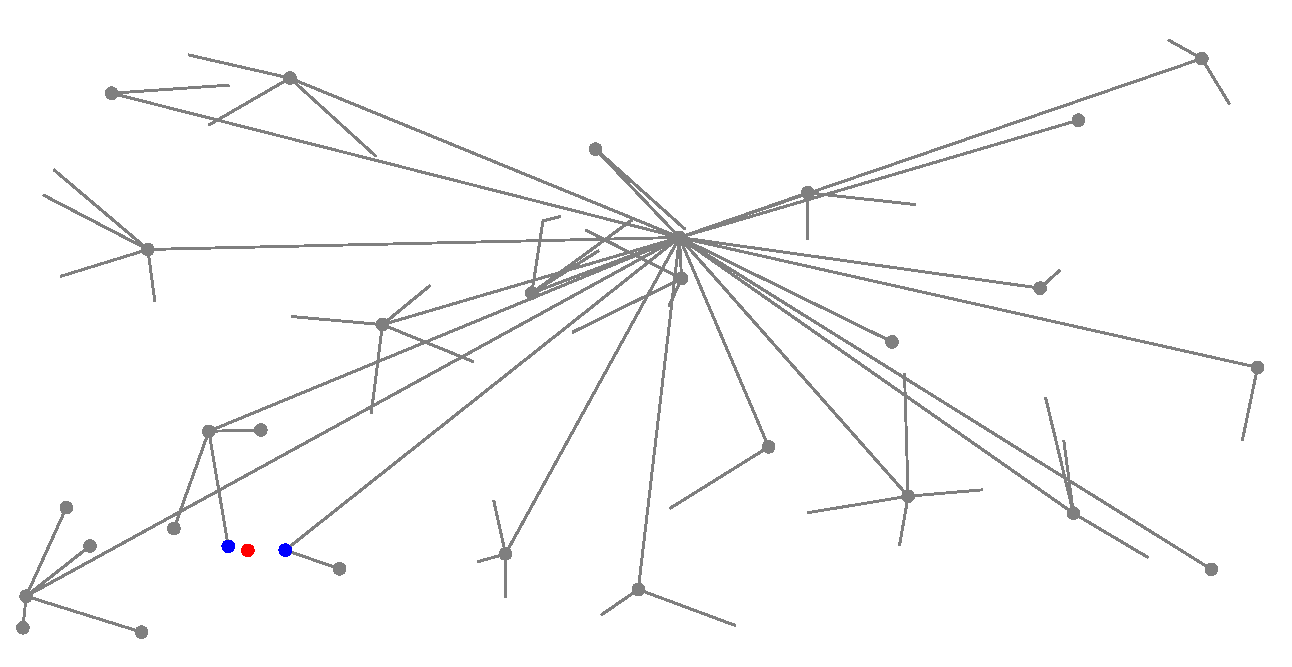
\includegraphics[width=110mm]{metric-tree.eps}}

The above drawing shows a cloud of (randomly generated) points in $ \RR^2 $ organized in a
{\codett MetricTree}.
It also illustrates the process of {\codett find\_close\_neighbours\_of} a given point.
This method takes two arguments : a {\codett Point} (drawn in red) and a distance.
It returns a list (drawn in blue) of all {\codett Node}s in the cloud which are close enough
to the red point (closer than the given distance).
It is irrelevant whether the red point belongs to the cloud or not;
if it belongs, it will be returned as element of the list.

The drawing above shows grey dots at nodes which have been analysed during the process of
{\codett find\_close\_neighbours} (their distance to the red dot has been computed).
Lines without a dot represent nodes in the {\codett MetricTree} which have not even been
looked at because their parent has decided (based on the triangular inequality)
that they cannot be close enough to the red dot.
Their distance to the red point has not been computed, thus alleviating the computational
burden.

If you want to run this example on your computer, it suffices to download three files,
({\codett Makefile}, {\codett main-\numb section 10.\numb parag 16.cpp} and
{\codett metric-tree-verbose.h})
from {\codett https://github.com/cristian-barbarosie/manifem/tree/master/src},
then {\codett make run-\numb section 10.\numb parag 16}.


\paragraph{\numb section 10.\numb parag 17. The cloud in progressive mesh generation}

The use of {\codett MetricTree} for progressive mesh generation (described in paragraph
\numb section 11.\numb parag 5, with examples in section \numb section 3)
is tricky when we are meshing a submanifold of $ \RR^n $
(a curve in $ \RR^2 $ or $ \RR^3 $, a surface in $ \RR^3 $)
because there are two distances we must deal with.
There is the global, Euclidian, distance in the surrounding space
and there is the local distance on the tangent space of the manifold.
They are equal locally (at short distances) unless we attach a specific Riemann metric
to the manifold as shown in paragraphs \numb section 3.\numb parag 23 and
\numb section 3.\numb parag 24.

Even if we don't play with a specific Riemann metric, the Euclidian metric is different,
at large distances, from the metric on the manifold defined by means of geodesics.
And anyway, computing the distance by means of geodesics is not affordable (it is too heavy
computationally).

We have chosen the following work-out.
We use a {\codett MetricTree} with (the square of) the usual Euclidian distance (which is
computationally cheap).
This means that a call to {\codett MetricTree::find\_close\_neighbours\_of} will produce a list
which is too large in the sense that it may contain points which are farther than the
distance given as argument.
The calling program must then filter this list by measuring distances with the local metric.
The difference shouldn't be important if we are careful to choose the {\codett
desired\_distance} (be it a constant or a function) small when compared with the curvature
of the manifold (see paragraph \numb section 3.\numb parag 16).

If we define a non-uniform Riemann metric (as in paragraph \numb section 3.\numb parag 23),
we must call {\codett find\_close\_neighbours\_of} with a modified value of the
distance.
If we define an anisotropic Riemann metric (as in paragraph \numb section 3.\numb parag 24),
we need a lower bound on the Rayleigh coefficient of the matrix $M$ (i.e.\ a lower bound
on its eigenvalues, or, equivalently, an upper bound of the spectral radius of the inverse
matrix) for computing the modified value to provide to {\codett find\_close\_neighbours\_of}.
Providing separately the {\codett principal\_part} and the {\codett deviatoric\_part} helps.
The {\codett principal\_part} is a positive scalar, while {\codett deviatoric\_part} is
a matrix responsible for the anisotropy; this matrix should be semi-definite positive.
Desirably, the {\codett deviatoric\_part} should be a singular matrix (having a null eigenvalue);
this way, the lower bound on the Rayleigh coefficient is simply the {\codett principal\_part}.
If we provide only the sum $M$, {\maniFEM} will compute, at each step, the lower bound on the
Rayleigh coefficient, which may be a heavy computational burden.
When the metric is highly anisotropic, the list returned by method
{\codett find\_close\_neighbours\_of} will be singnificantly larger than the correct, filtered, list.
